% Options for packages loaded elsewhere
\PassOptionsToPackage{unicode}{hyperref}
\PassOptionsToPackage{hyphens}{url}
\PassOptionsToPackage{dvipsnames,svgnames,x11names}{xcolor}
%
\documentclass[
  letterpaper,
  DIV=11,
  numbers=noendperiod]{scrartcl}

\usepackage{amsmath,amssymb}
\usepackage{iftex}
\ifPDFTeX
  \usepackage[T1]{fontenc}
  \usepackage[utf8]{inputenc}
  \usepackage{textcomp} % provide euro and other symbols
\else % if luatex or xetex
  \usepackage{unicode-math}
  \defaultfontfeatures{Scale=MatchLowercase}
  \defaultfontfeatures[\rmfamily]{Ligatures=TeX,Scale=1}
\fi
\usepackage{lmodern}
\ifPDFTeX\else  
    % xetex/luatex font selection
\fi
% Use upquote if available, for straight quotes in verbatim environments
\IfFileExists{upquote.sty}{\usepackage{upquote}}{}
\IfFileExists{microtype.sty}{% use microtype if available
  \usepackage[]{microtype}
  \UseMicrotypeSet[protrusion]{basicmath} % disable protrusion for tt fonts
}{}
\makeatletter
\@ifundefined{KOMAClassName}{% if non-KOMA class
  \IfFileExists{parskip.sty}{%
    \usepackage{parskip}
  }{% else
    \setlength{\parindent}{0pt}
    \setlength{\parskip}{6pt plus 2pt minus 1pt}}
}{% if KOMA class
  \KOMAoptions{parskip=half}}
\makeatother
\usepackage{xcolor}
\setlength{\emergencystretch}{3em} % prevent overfull lines
\setcounter{secnumdepth}{-\maxdimen} % remove section numbering
% Make \paragraph and \subparagraph free-standing
\makeatletter
\ifx\paragraph\undefined\else
  \let\oldparagraph\paragraph
  \renewcommand{\paragraph}{
    \@ifstar
      \xxxParagraphStar
      \xxxParagraphNoStar
  }
  \newcommand{\xxxParagraphStar}[1]{\oldparagraph*{#1}\mbox{}}
  \newcommand{\xxxParagraphNoStar}[1]{\oldparagraph{#1}\mbox{}}
\fi
\ifx\subparagraph\undefined\else
  \let\oldsubparagraph\subparagraph
  \renewcommand{\subparagraph}{
    \@ifstar
      \xxxSubParagraphStar
      \xxxSubParagraphNoStar
  }
  \newcommand{\xxxSubParagraphStar}[1]{\oldsubparagraph*{#1}\mbox{}}
  \newcommand{\xxxSubParagraphNoStar}[1]{\oldsubparagraph{#1}\mbox{}}
\fi
\makeatother


\providecommand{\tightlist}{%
  \setlength{\itemsep}{0pt}\setlength{\parskip}{0pt}}\usepackage{longtable,booktabs,array}
\usepackage{calc} % for calculating minipage widths
% Correct order of tables after \paragraph or \subparagraph
\usepackage{etoolbox}
\makeatletter
\patchcmd\longtable{\par}{\if@noskipsec\mbox{}\fi\par}{}{}
\makeatother
% Allow footnotes in longtable head/foot
\IfFileExists{footnotehyper.sty}{\usepackage{footnotehyper}}{\usepackage{footnote}}
\makesavenoteenv{longtable}
\usepackage{graphicx}
\makeatletter
\newsavebox\pandoc@box
\newcommand*\pandocbounded[1]{% scales image to fit in text height/width
  \sbox\pandoc@box{#1}%
  \Gscale@div\@tempa{\textheight}{\dimexpr\ht\pandoc@box+\dp\pandoc@box\relax}%
  \Gscale@div\@tempb{\linewidth}{\wd\pandoc@box}%
  \ifdim\@tempb\p@<\@tempa\p@\let\@tempa\@tempb\fi% select the smaller of both
  \ifdim\@tempa\p@<\p@\scalebox{\@tempa}{\usebox\pandoc@box}%
  \else\usebox{\pandoc@box}%
  \fi%
}
% Set default figure placement to htbp
\def\fps@figure{htbp}
\makeatother

\usepackage{booktabs}
\usepackage{longtable}
\usepackage{array}
\usepackage{multirow}
\usepackage{wrapfig}
\usepackage{float}
\usepackage{colortbl}
\usepackage{pdflscape}
\usepackage{tabu}
\usepackage{threeparttable}
\usepackage{threeparttablex}
\usepackage[normalem]{ulem}
\usepackage{makecell}
\usepackage{xcolor}
\usepackage{caption}
\usepackage{anyfontsize}
\KOMAoption{captions}{tableheading}
\makeatletter
\@ifpackageloaded{caption}{}{\usepackage{caption}}
\AtBeginDocument{%
\ifdefined\contentsname
  \renewcommand*\contentsname{Table of contents}
\else
  \newcommand\contentsname{Table of contents}
\fi
\ifdefined\listfigurename
  \renewcommand*\listfigurename{List of Figures}
\else
  \newcommand\listfigurename{List of Figures}
\fi
\ifdefined\listtablename
  \renewcommand*\listtablename{List of Tables}
\else
  \newcommand\listtablename{List of Tables}
\fi
\ifdefined\figurename
  \renewcommand*\figurename{Figure}
\else
  \newcommand\figurename{Figure}
\fi
\ifdefined\tablename
  \renewcommand*\tablename{Table}
\else
  \newcommand\tablename{Table}
\fi
}
\@ifpackageloaded{float}{}{\usepackage{float}}
\floatstyle{ruled}
\@ifundefined{c@chapter}{\newfloat{codelisting}{h}{lop}}{\newfloat{codelisting}{h}{lop}[chapter]}
\floatname{codelisting}{Listing}
\newcommand*\listoflistings{\listof{codelisting}{List of Listings}}
\makeatother
\makeatletter
\makeatother
\makeatletter
\@ifpackageloaded{caption}{}{\usepackage{caption}}
\@ifpackageloaded{subcaption}{}{\usepackage{subcaption}}
\makeatother

\usepackage{bookmark}

\IfFileExists{xurl.sty}{\usepackage{xurl}}{} % add URL line breaks if available
\urlstyle{same} % disable monospaced font for URLs
\hypersetup{
  pdftitle={American Samoa Model Checks},
  pdfauthor={Marc Nadon and Meg Oshima},
  colorlinks=true,
  linkcolor={blue},
  filecolor={Maroon},
  citecolor={Blue},
  urlcolor={Blue},
  pdfcreator={LaTeX via pandoc}}


\title{American Samoa Model Checks}
\author{Marc Nadon and Meg Oshima}
\date{2026-02-13}

\begin{document}
\maketitle


\textbf{This is a summary report for the APRU base model run.}

\section{Model Output}\label{model-output}

\subsection{Input Data}

\pandocbounded{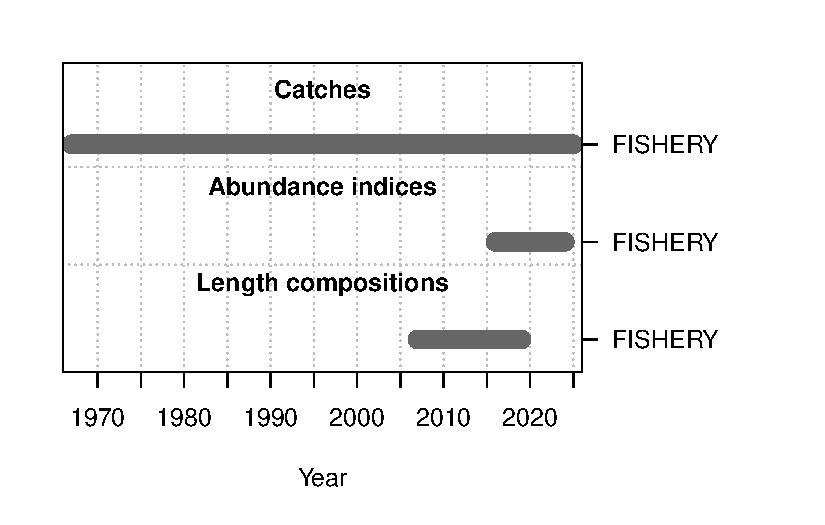
\includegraphics[keepaspectratio]{APRU_005_2025_endyr_Marc_model_diags_report_files/figure-pdf/dataplot-1.pdf}}

\pandocbounded{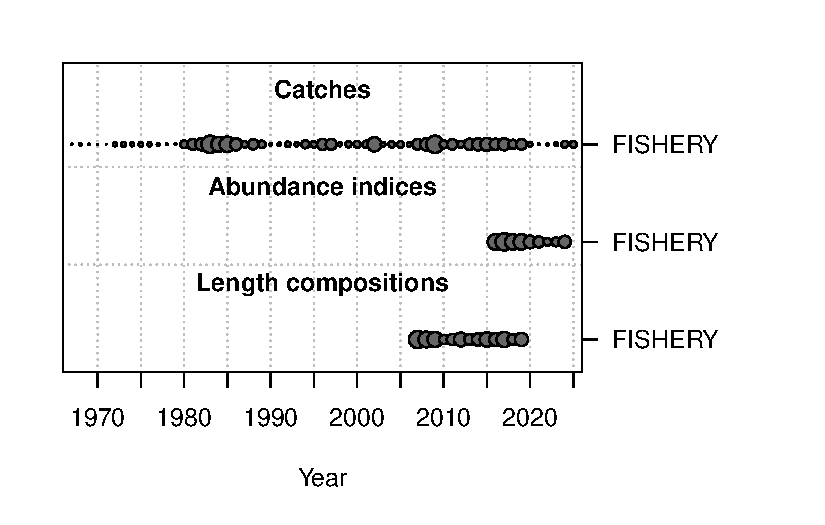
\includegraphics[keepaspectratio]{APRU_005_2025_endyr_Marc_model_diags_report_files/figure-pdf/dataplot-2.pdf}}

\subsection{Convergence Check}

\begin{verbatim}
  Converged     MaxGrad
1      TRUE 6.94896e-05
\end{verbatim}

\begin{verbatim}
[1] "1 NOTE:  Max data length bin: 90  < max pop len bins: 100; so will accumulate larger pop len bins"
[2] "N warnings: 1"                                                                                    
\end{verbatim}

\subsection{Fit to Model}

\subsubsection{CPUE}\label{cpue}

\begin{table}
\fontsize{12.0pt}{14.4pt}\selectfont
\begin{tabular*}{\linewidth}{@{\extracolsep{\fill}}lrr}
\toprule
Fleet & RMSE.perc & Nobs \\ 
\midrule\addlinespace[2.5pt]
FISHERY & 93.3 & 9 \\ 
Combined & 93.3 & 9 \\ 
\bottomrule
\end{tabular*}
\end{table}

\begin{center}
\pandocbounded{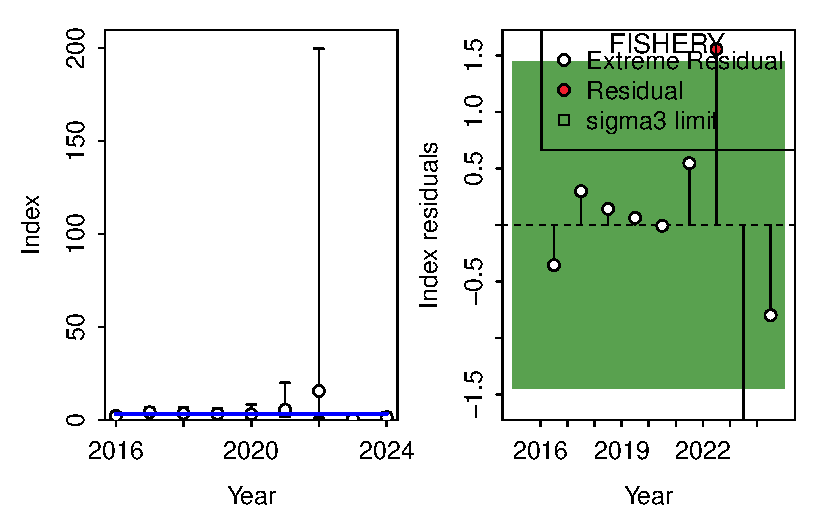
\includegraphics[keepaspectratio]{APRU_005_2025_endyr_Marc_model_diags_report_files/figure-pdf/indexfits-1.pdf}}
\end{center}

\subsubsection{Length Comp}\label{length-comp}

\begin{table}
\fontsize{12.0pt}{14.4pt}\selectfont
\begin{tabular*}{\linewidth}{@{\extracolsep{\fill}}lrr}
\toprule
Fleet & RMSE.perc & Nobs \\ 
\midrule\addlinespace[2.5pt]
FISHERY & 4.5 & 13 \\ 
Combined & 4.5 & 13 \\ 
\bottomrule
\end{tabular*}
\end{table}

\begin{figure}

\begin{minipage}{0.50\linewidth}

\begin{verbatim}
        w        lo        hi 
0.4913593 0.2792918 1.5851703 
\end{verbatim}

\end{minipage}%
%
\begin{minipage}{0.50\linewidth}

\begin{verbatim}
    Index runs.p   test  sigma3.lo sigma3.hi type
1 FISHERY  0.623 Passed -0.1462169 0.1462169  len
\end{verbatim}

\end{minipage}%
\newline
\begin{minipage}{0.50\linewidth}
\begin{center}
\pandocbounded{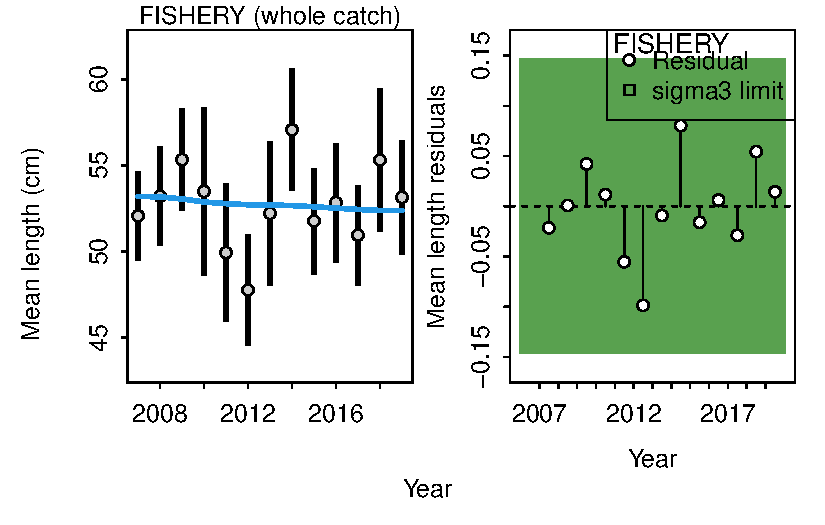
\includegraphics[keepaspectratio]{APRU_005_2025_endyr_Marc_model_diags_report_files/figure-pdf/lenfits-1.pdf}}
\end{center}
\end{minipage}%

\end{figure}%

\begin{center}
\pandocbounded{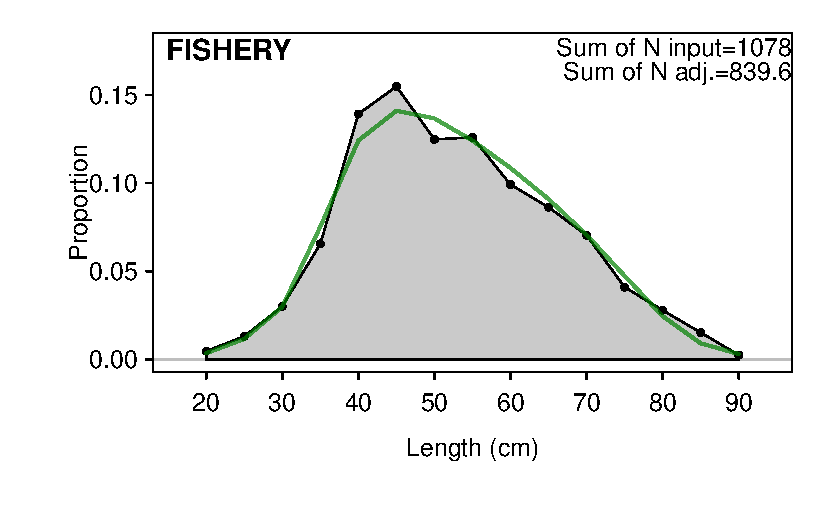
\includegraphics[keepaspectratio]{APRU_005_2025_endyr_Marc_model_diags_report_files/figure-pdf/lencompfits-1.pdf}}
\end{center}

\begin{center}
\pandocbounded{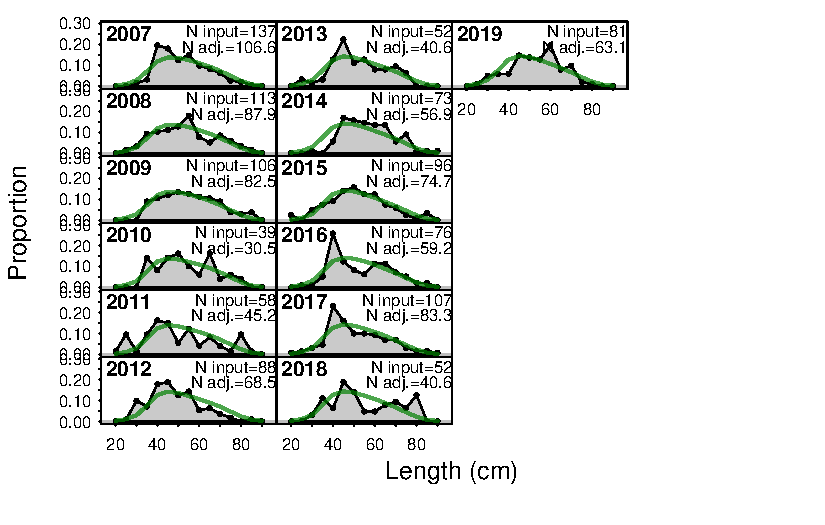
\includegraphics[keepaspectratio]{APRU_005_2025_endyr_Marc_model_diags_report_files/figure-pdf/lencompfits-2.pdf}}
\end{center}

\subsection{Retrospective and Hindcasting}

\subsubsection{Retrospective}\label{retrospective}

\begin{verbatim}
[1] "No retrospective runs were found"
\end{verbatim}

\subsubsection{Hindcasting}\label{hindcasting}

\begin{verbatim}
[1] "No information for hindcast was found"
\end{verbatim}

\subsection{Recruitment Deviations}

\subsection{Likelihood Profile}

\begin{verbatim}
[1] "No likelihood runs were found"
\end{verbatim}

\subsection{Management Quantities}

\begin{verbatim}

 starter.sso with Bratio: SSB/SSBMSY and F: _abs_F 
 
\end{verbatim}

\pandocbounded{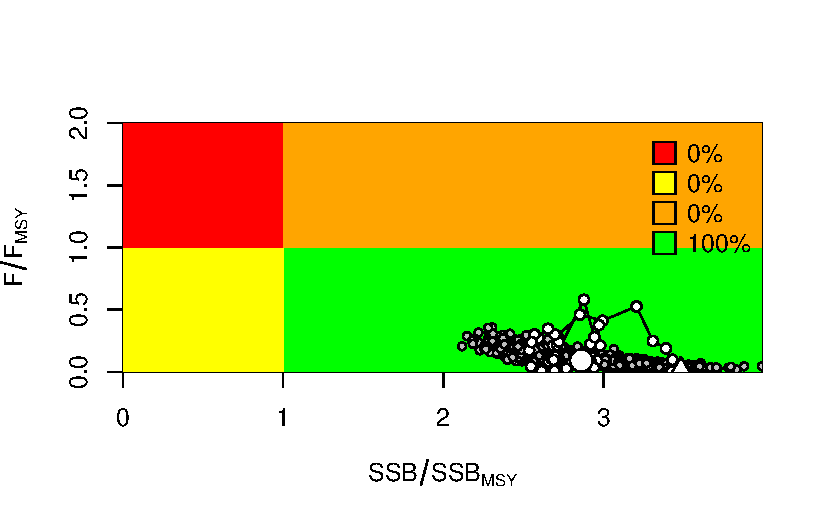
\includegraphics[keepaspectratio]{APRU_005_2025_endyr_Marc_model_diags_report_files/figure-pdf/mvlnkb-1.pdf}}

\pandocbounded{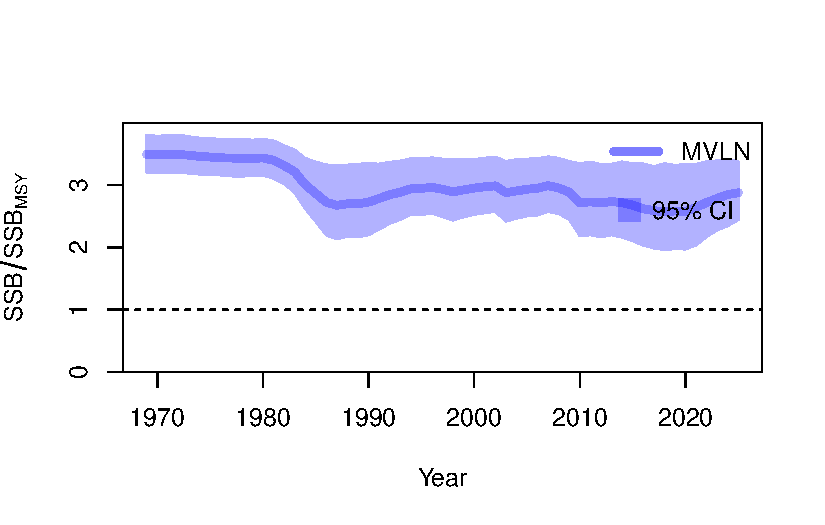
\includegraphics[keepaspectratio]{APRU_005_2025_endyr_Marc_model_diags_report_files/figure-pdf/mvlnkb-2.pdf}}

\pandocbounded{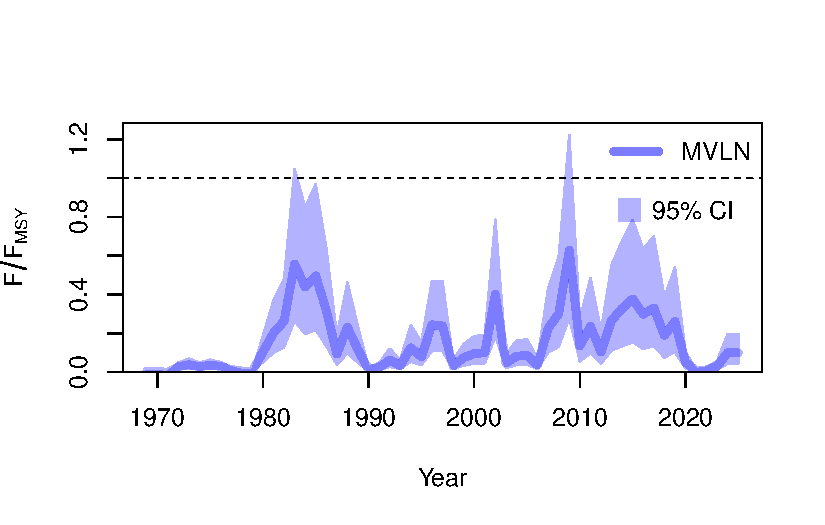
\includegraphics[keepaspectratio]{APRU_005_2025_endyr_Marc_model_diags_report_files/figure-pdf/mvlnkb-3.pdf}}

\pandocbounded{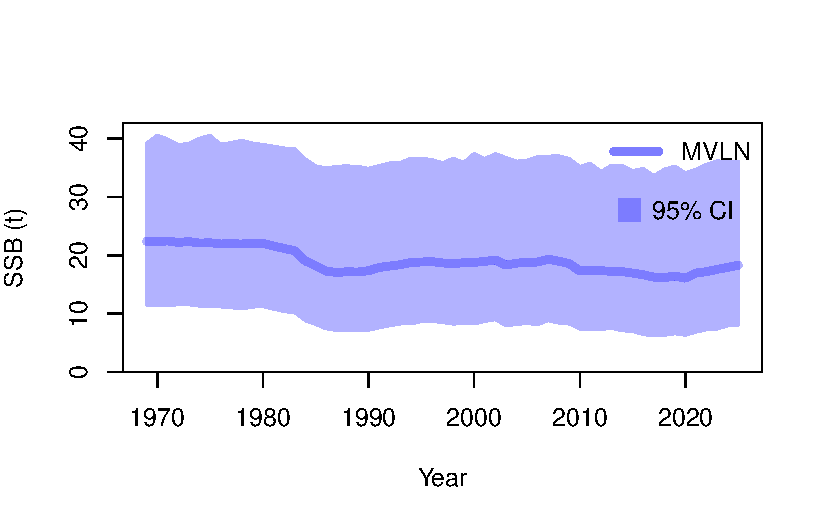
\includegraphics[keepaspectratio]{APRU_005_2025_endyr_Marc_model_diags_report_files/figure-pdf/mvlnkb-4.pdf}}

\pandocbounded{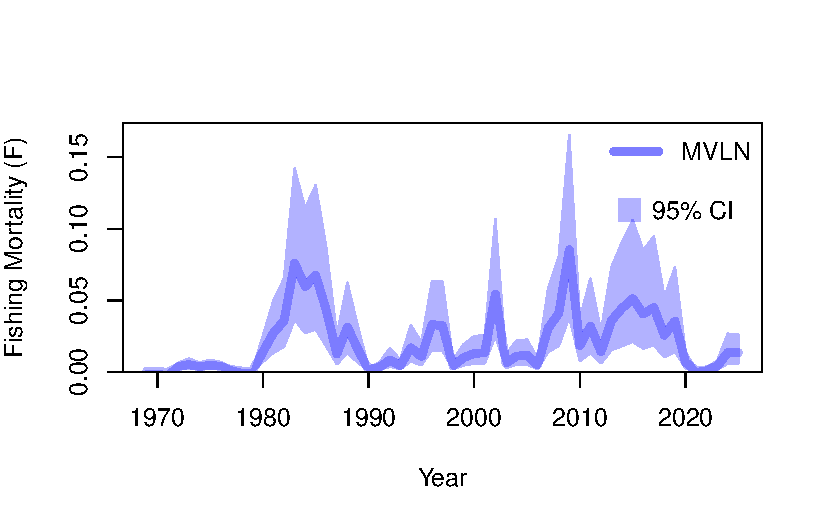
\includegraphics[keepaspectratio]{APRU_005_2025_endyr_Marc_model_diags_report_files/figure-pdf/mvlnkb-5.pdf}}

\begin{verbatim}
null device 
          1 
\end{verbatim}

\subsection{Jitter}

\begin{verbatim}
[1] "No jitter runs were found."
\end{verbatim}

\subsection{Selectivity and Maturity}

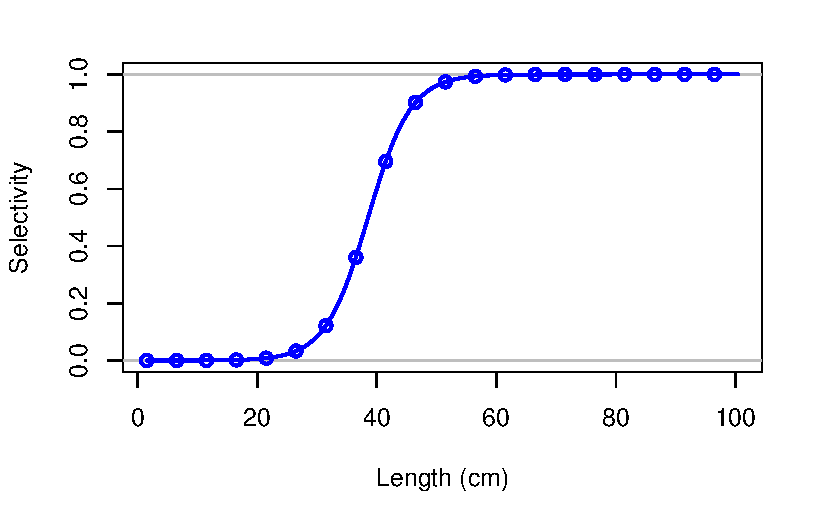
\includegraphics[width=7.4cm,height=\textheight,keepaspectratio]{APRU_005_2025_endyr_Marc_model_diags_report_files/figure-pdf/selectivity-1.pdf}

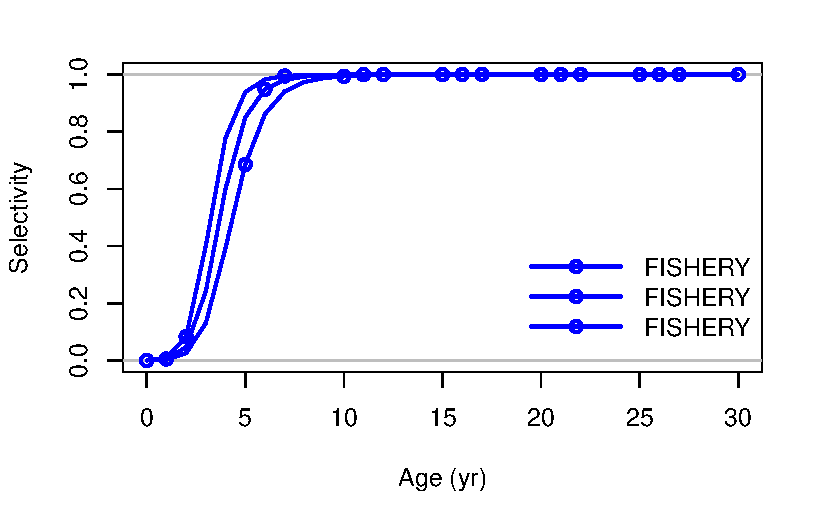
\includegraphics[width=7.4cm,height=\textheight,keepaspectratio]{APRU_005_2025_endyr_Marc_model_diags_report_files/figure-pdf/selectivity-2.pdf}

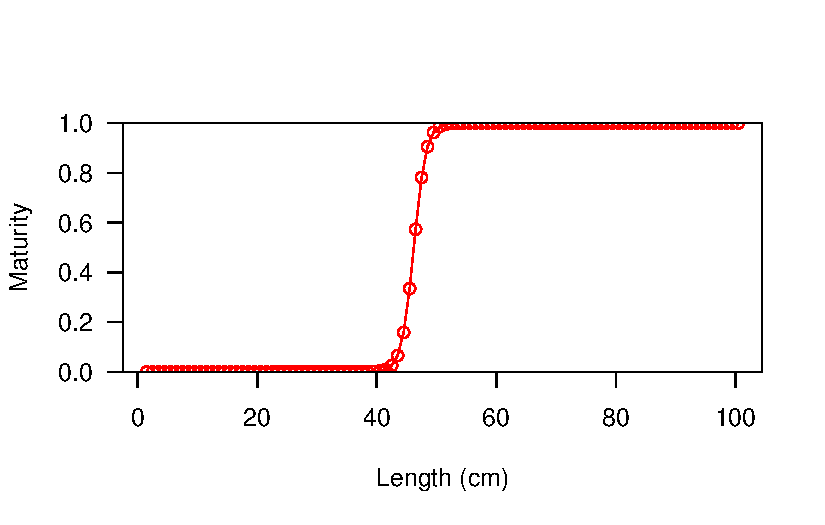
\includegraphics[width=7.2cm,height=\textheight,keepaspectratio]{APRU_005_2025_endyr_Marc_model_diags_report_files/figure-pdf/maturity-1.pdf}

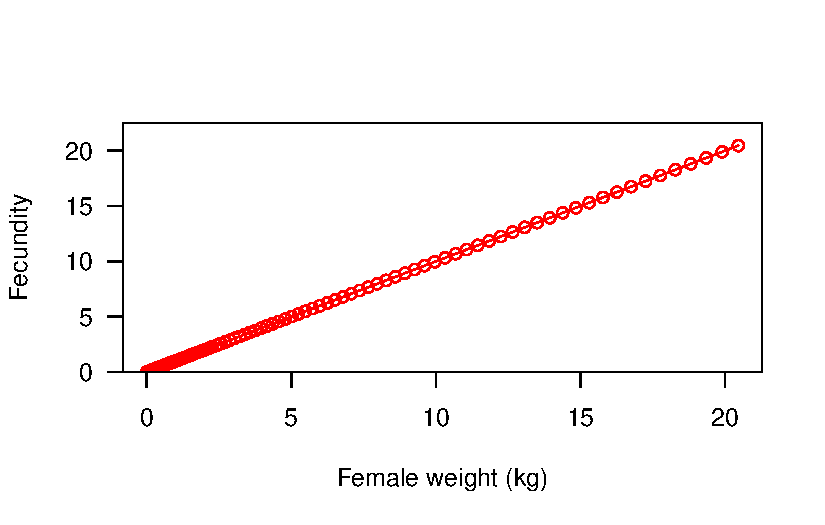
\includegraphics[width=7.2cm,height=\textheight,keepaspectratio]{APRU_005_2025_endyr_Marc_model_diags_report_files/figure-pdf/maturity-2.pdf}




\end{document}
